%
% Diskussion und Bewertung
%
\section{Experimente und Auswertung}
Das hier vorgestellte und implementierte Verfahren wurde genutzt um acht verschiedene Filter bestehend aus SMARTS-Ausdr�cken miteinander zu vergleichen. Diese Filter wurden von im Rahmen der Datenbank ChEMBL \cite{ChEMBL} aus den folgenen Quellen zusammengetragen:
\begin{enumerate}
	\item Bristol-Myers Squibb HTS Deck Filters (\textbf{BMS})
	\item SureChEMBL Data (\textbf{SureChEMBL})
	\item Pan Assay Interference Compounds Filters (\textbf{PAINS})
	\item Glaxo Wellcome Hard Filters (\textbf{Glaxo})
	\item University of Dundee NTD Screening Library Filters (\textbf{Dundee})
	\item Inpharmatica Unwanted Fragments (\textbf{Inpharmatica})
	\item NIH MLSMR Excluded Functionality Filters (\textbf{MLSMR})
	\item Pfizer LINT filters (\textbf{LINT})
\end{enumerate} 

Die gewonnenen Listen bestehend aus SMARTS-Ausdr�cken wurden von Christian Laggner auf falsche SMARTS-Ausdr�cke untersucht und diese korrigiert (siehe Anhang \ref{ssec:experiments}).
Sie werden als sogenannte \textit{structural alerts} eingesetzt. Solche \textit{structural alerts} werden genutzt um unter Umst�nden problematische Molek�le bei der Wirkstoffentwicklung herauszufiltern. So werden Molek�le mit toxikologisch Substrukturen oder funktionellen Gruppen ausgefiltert, aber auch bekannte instabile Molek�le, Molek�le, die bei Tests st�ren k�nnten und welche, die beim HTS (\textit{High throughput Screening}) \cite{chemoinformatik} h�ufige Treffer darstellen. \cite{ChEMBLrelease}

\begin{table}[h]
	\centering
	\captionabove{�bersicht �ber die Anzahl der SMARTS-Ausdr�cke pro \textit{structural alert}-Filter vor und nach der �bergabe an das Programm \textit{SmartsSmarts} (siehe Kapitel \ref{ssec:vorverarbeitung}) des Verfahrens.}
	\begin{tabular}{| l | l | l |}
		\hline Filter-Set & Anzahl & nach �bergabe\\
		& SMARTS-Ausdr�cke & an \textit{SmartsSmarts}\\
		\hline BMS & 179 & 87\\
		Dundee & 104 & 100\\
		Glaxo & 54 & 54\\
		Inpharmatica & 91 & 83\\
		LINT & 57 & 48\\
		MLSMR & 115 & 105\\
		PAINS & 480 & 423\\
		SureChEMBL & 165 & 148\\ \hline
	\end{tabular}
	\label{tab:experiments}
\end{table}

\newpage
\begin{figure}[h!]
\fbox{\begin{minipage}{16cm}
	\begin{center}
	\begin{minipage}{5cm}
		\centering
		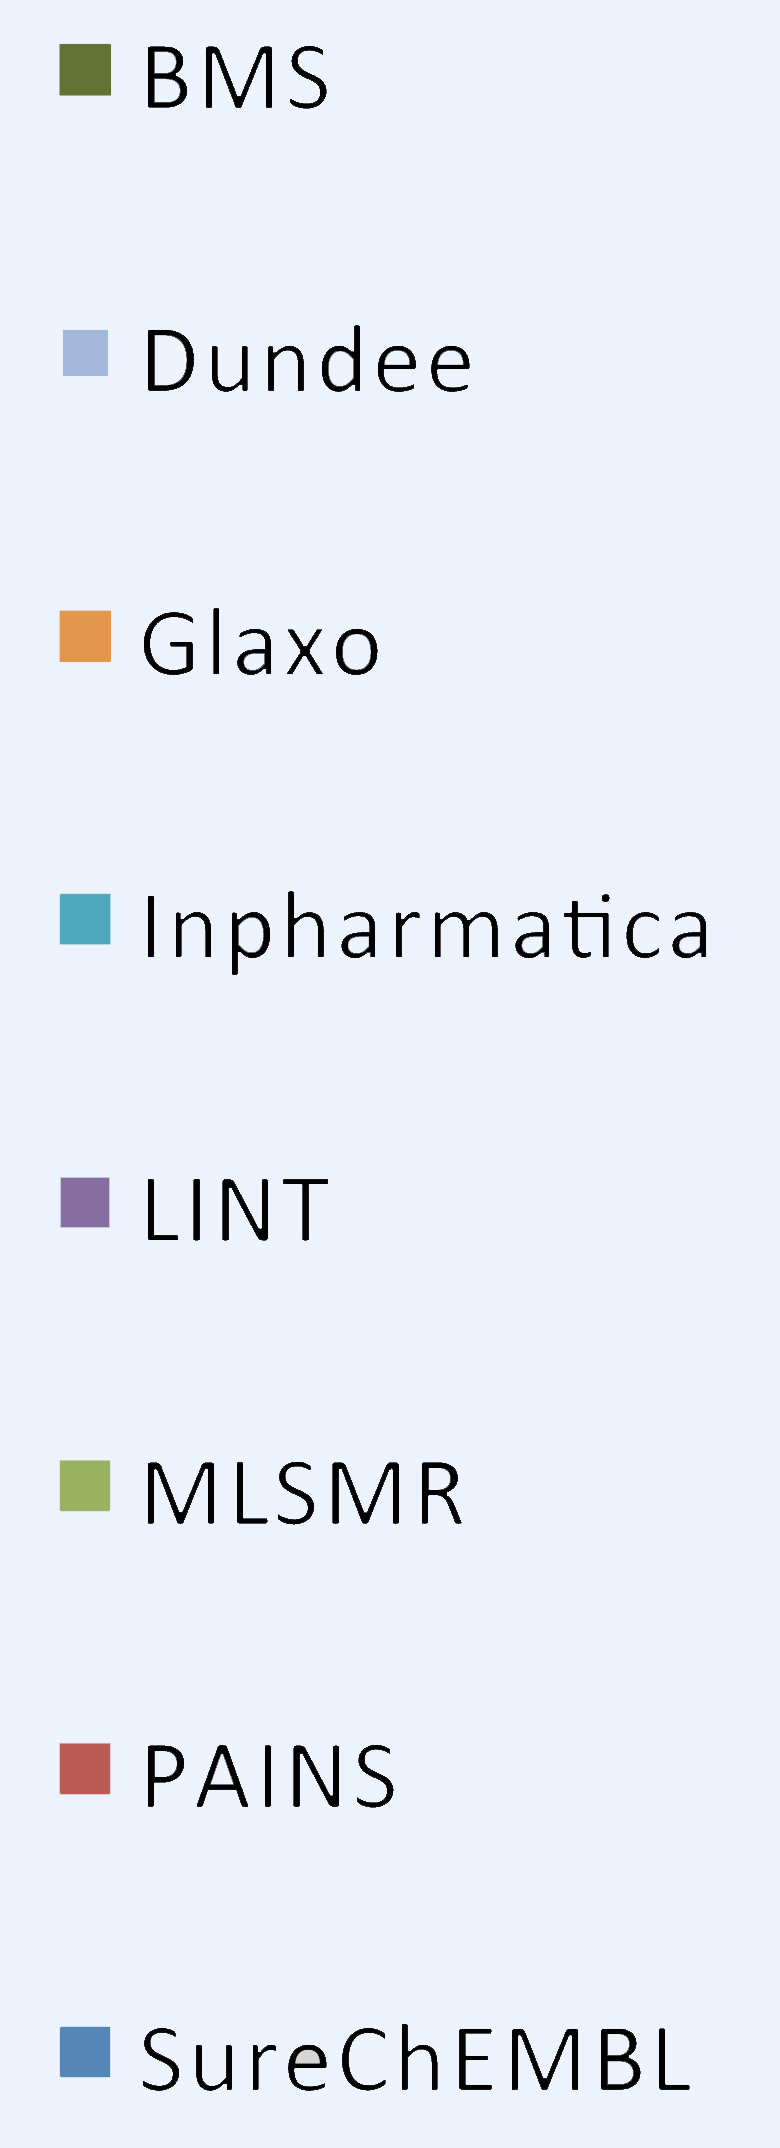
\includegraphics[width=3cm]{images/Legende3}
	\end{minipage}
	\begin{minipage}{5cm}
		\centering
		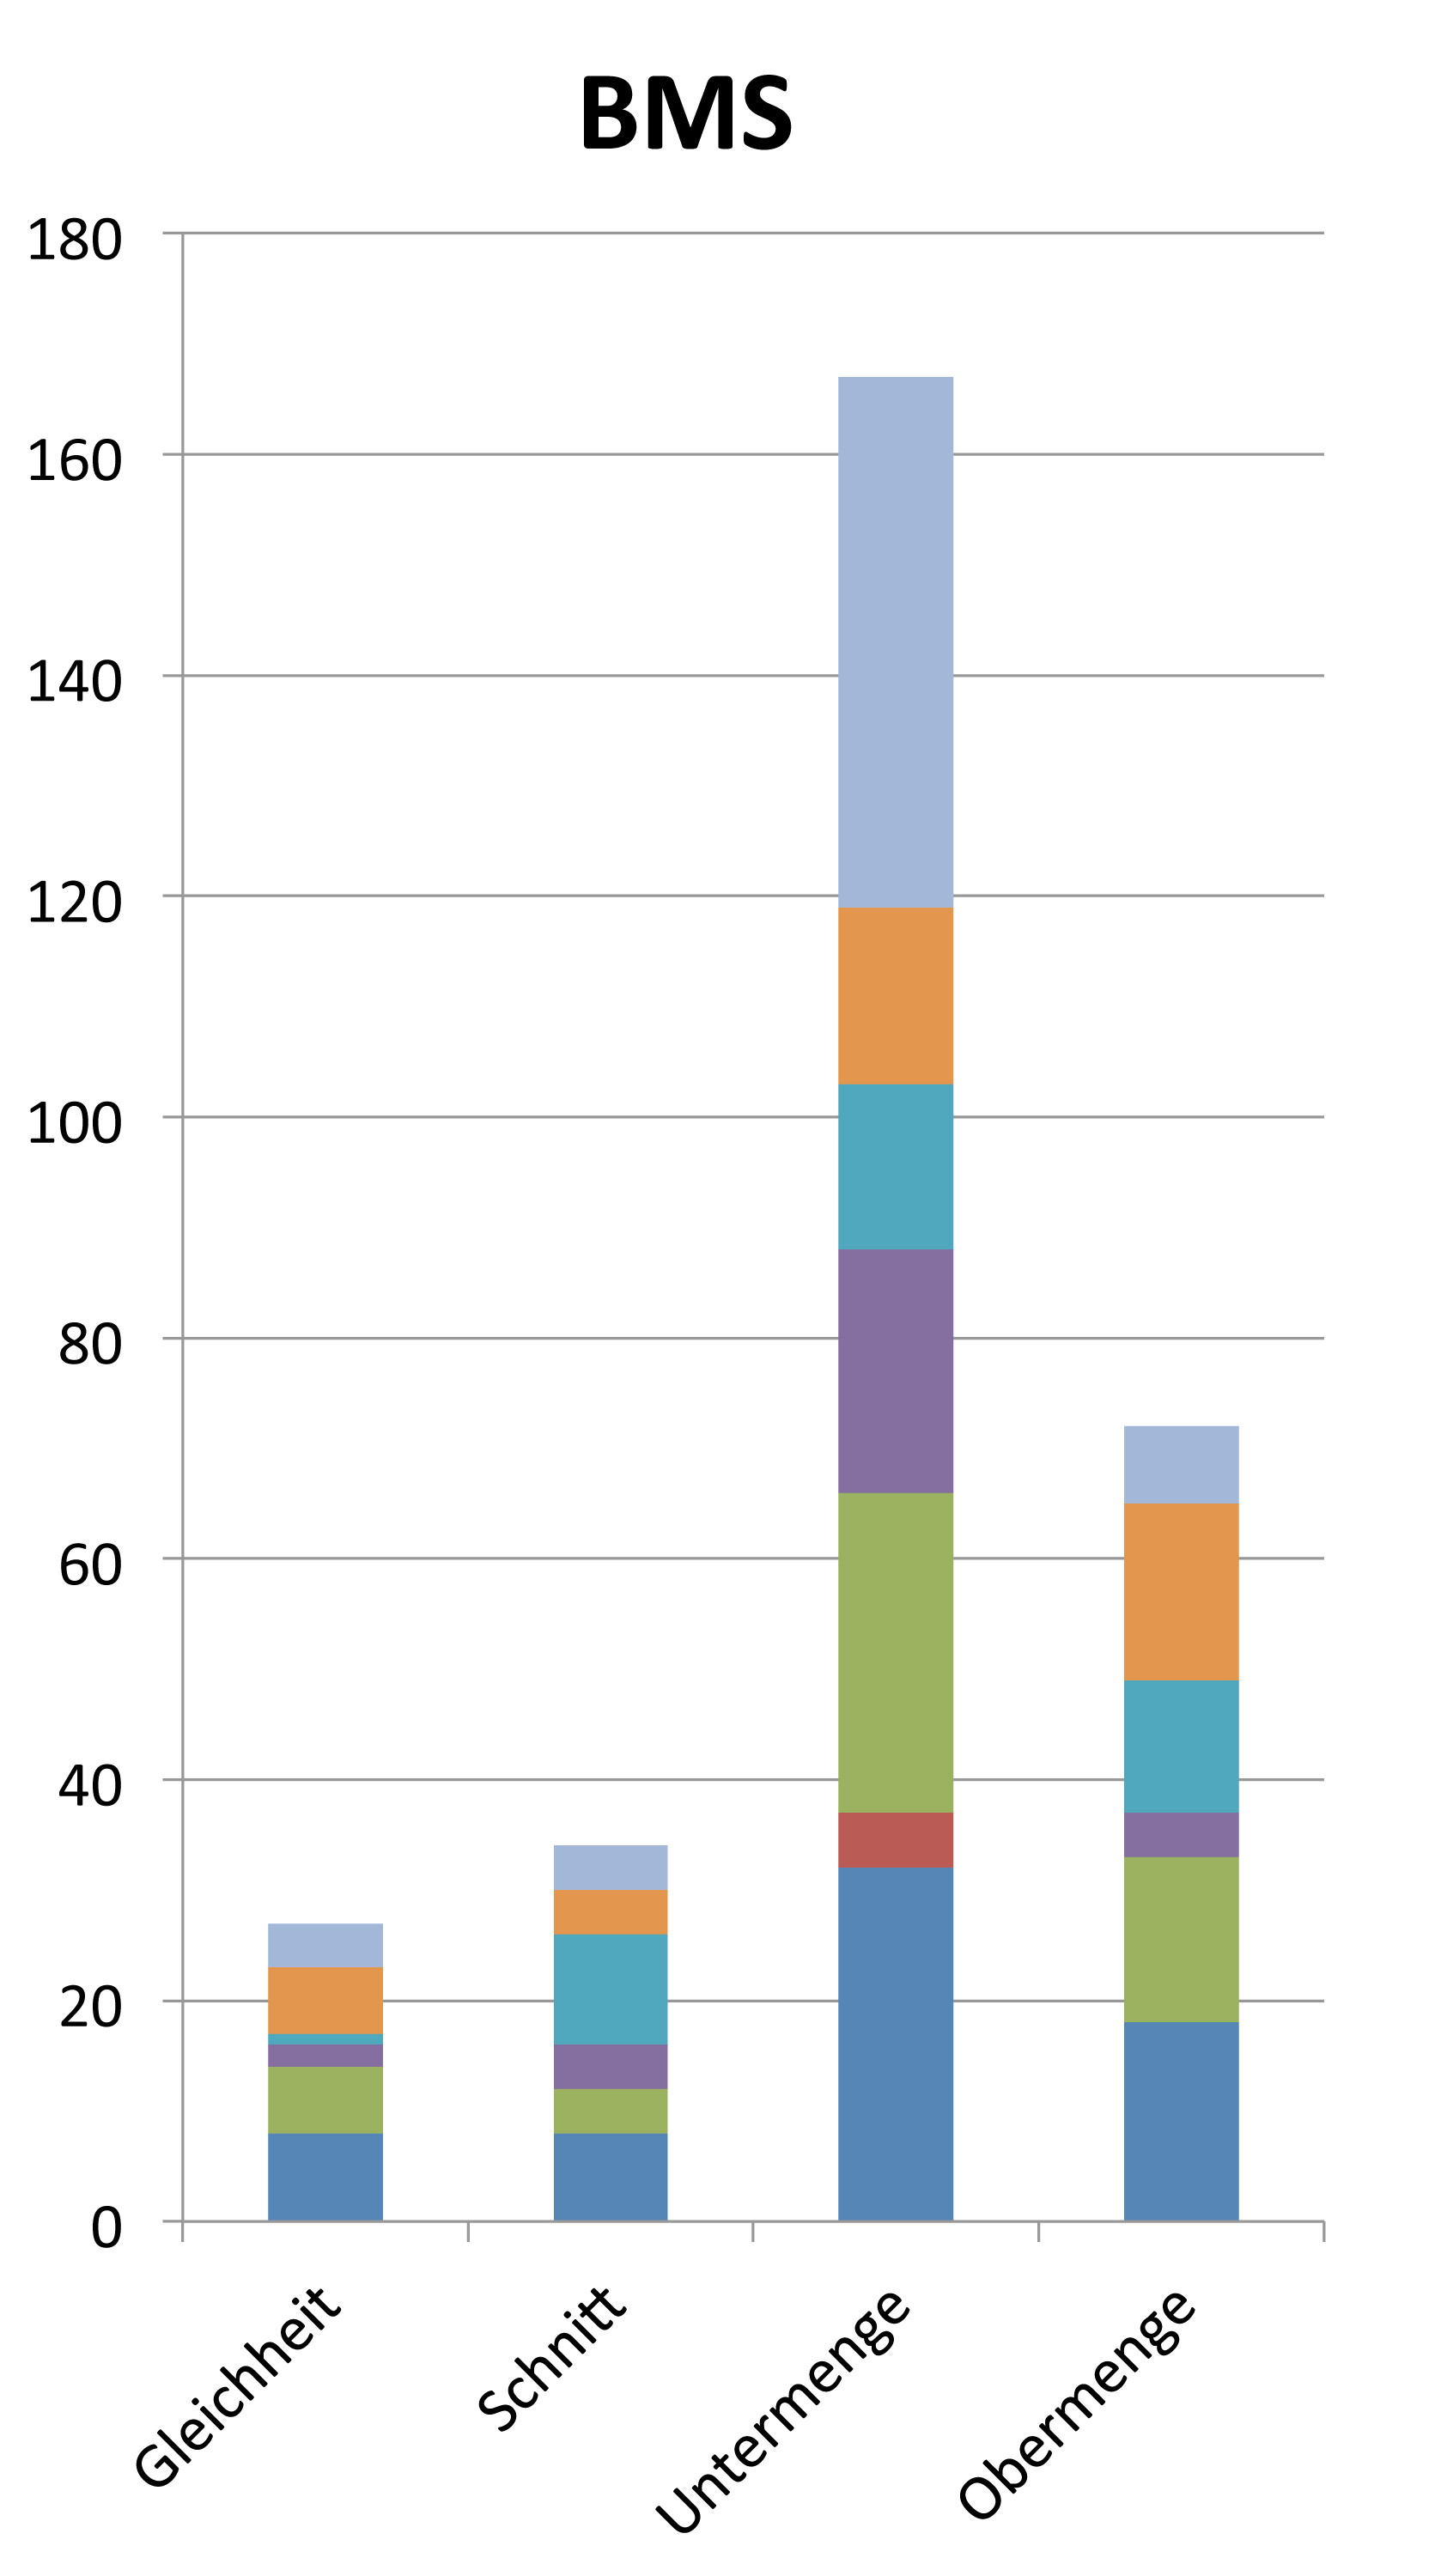
\includegraphics[width=5cm]{images/BMS}
	\end{minipage}
	\begin{minipage}{5cm}
		\centering
		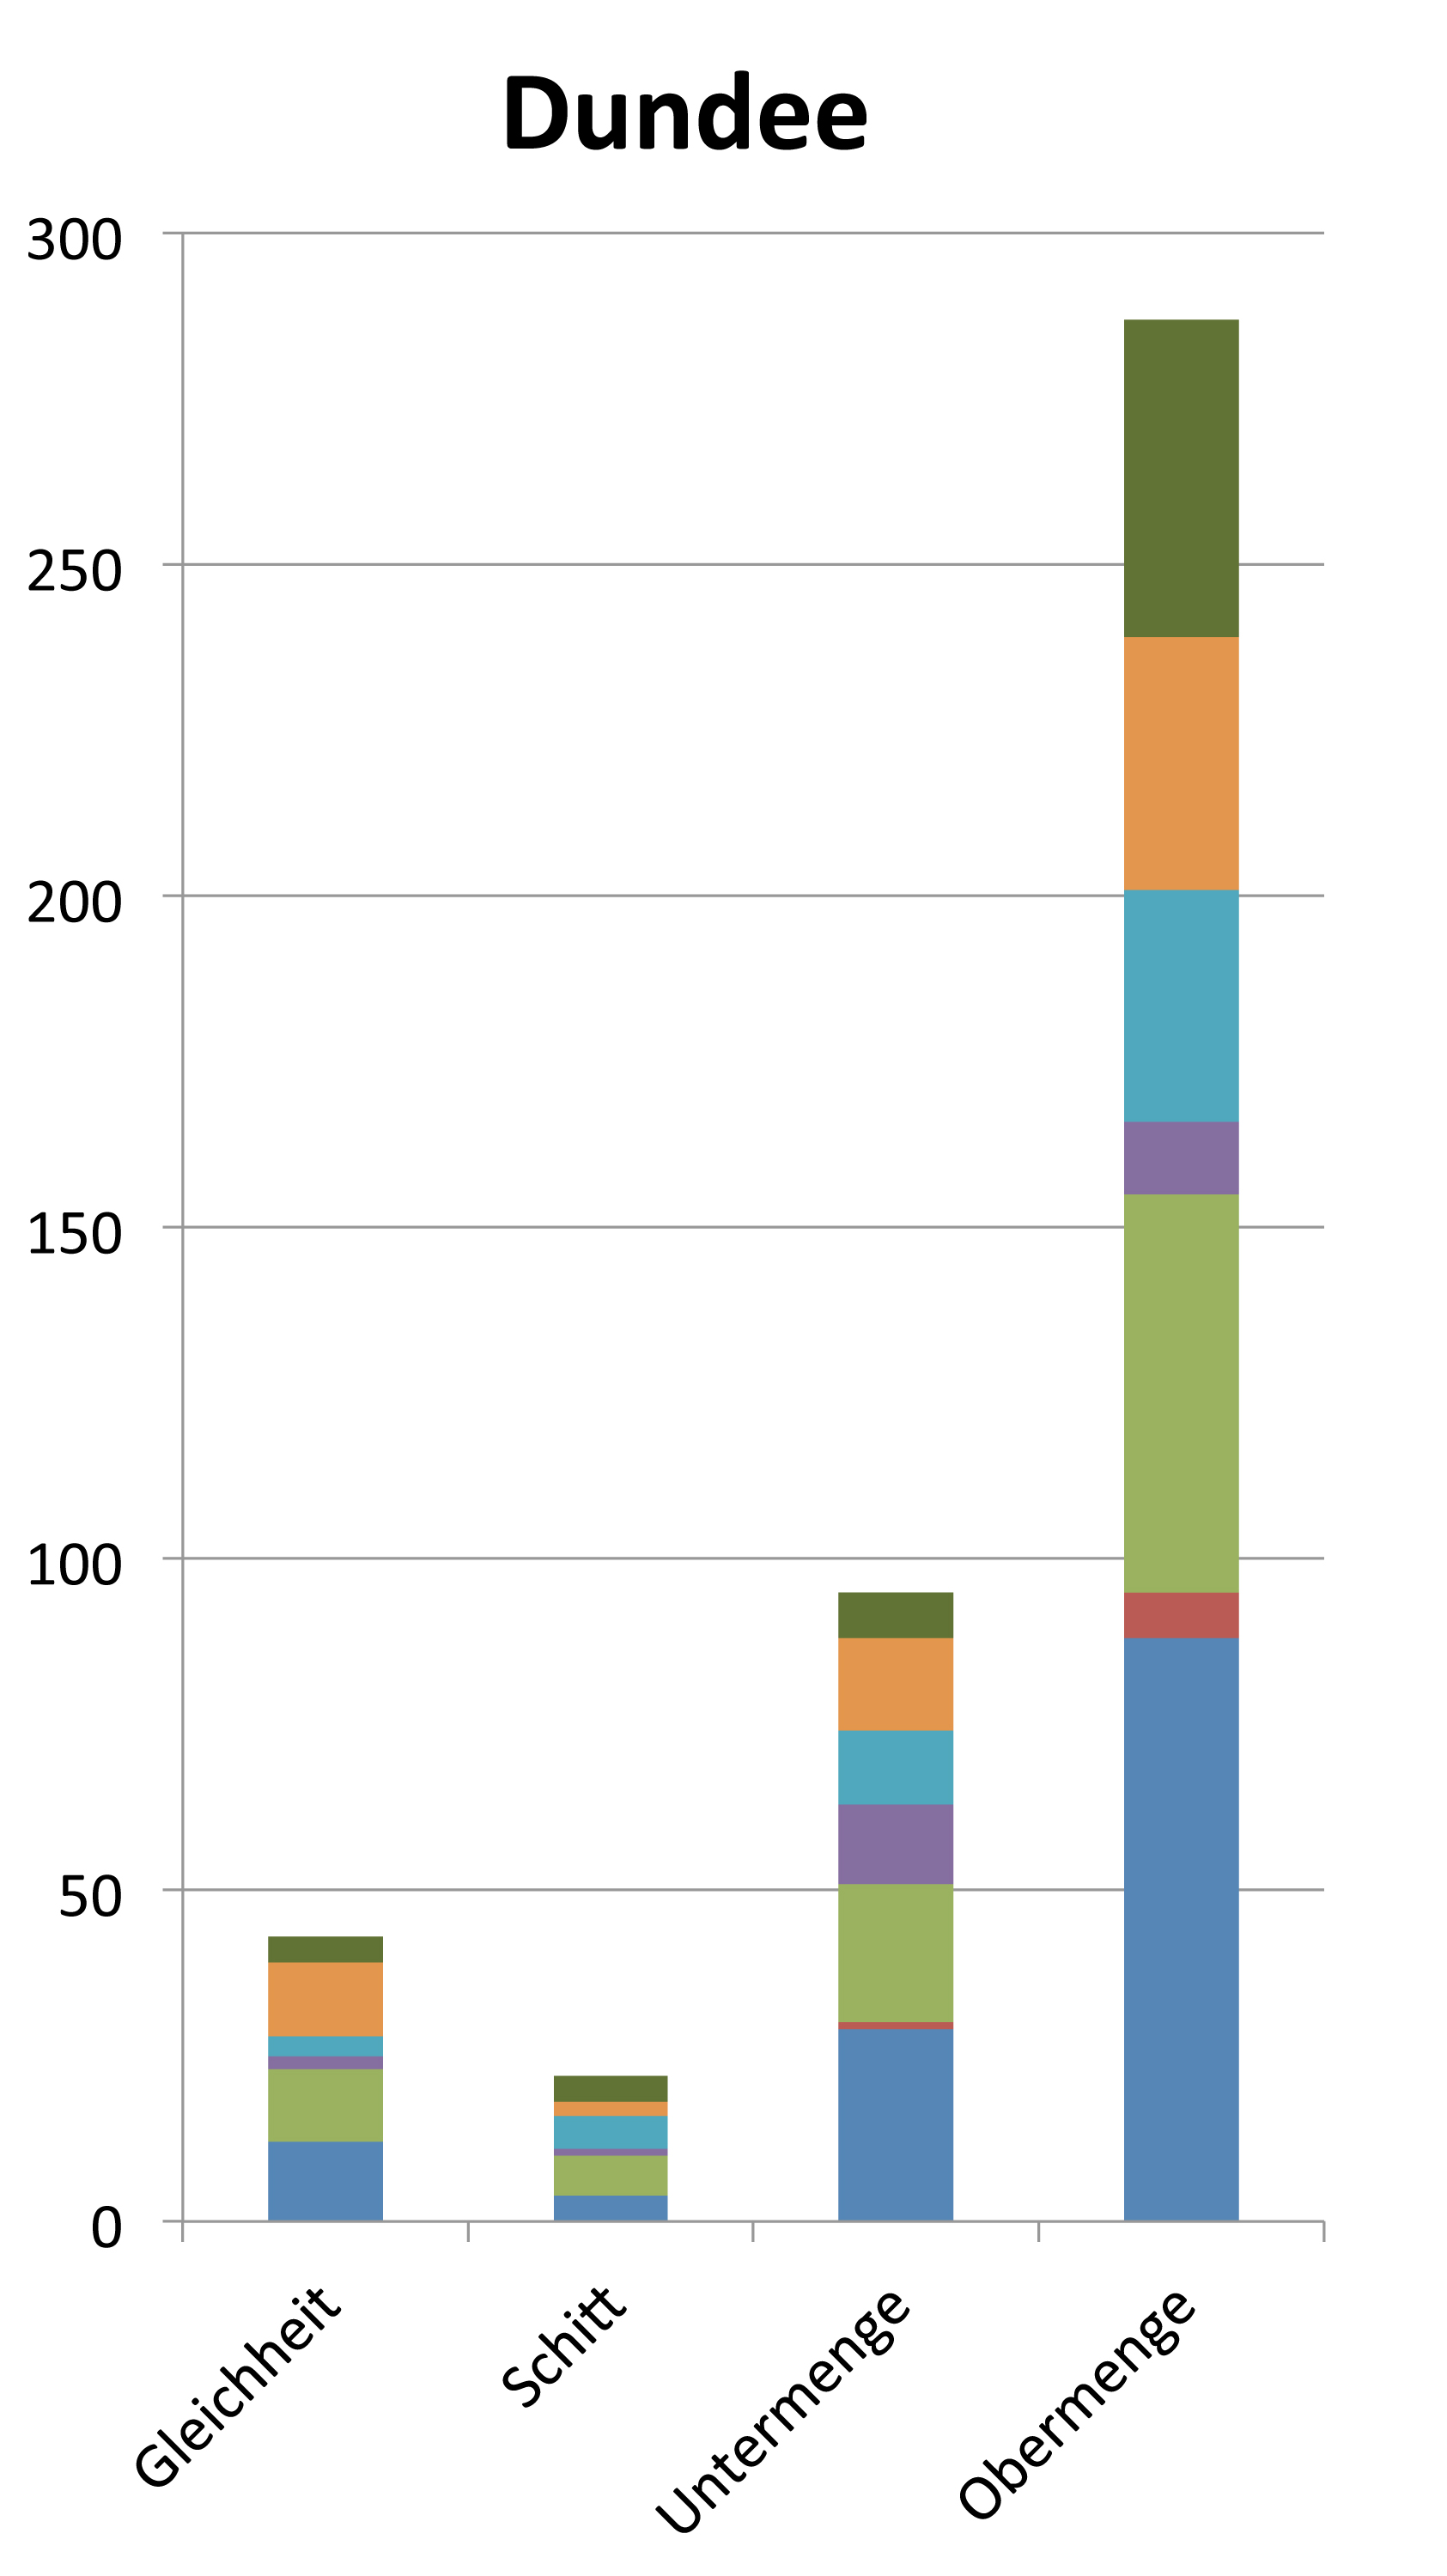
\includegraphics[width=5cm]{images/Dundee}
	\end{minipage}
\begin{center}
	\begin{minipage}{7cm}
		\centering
		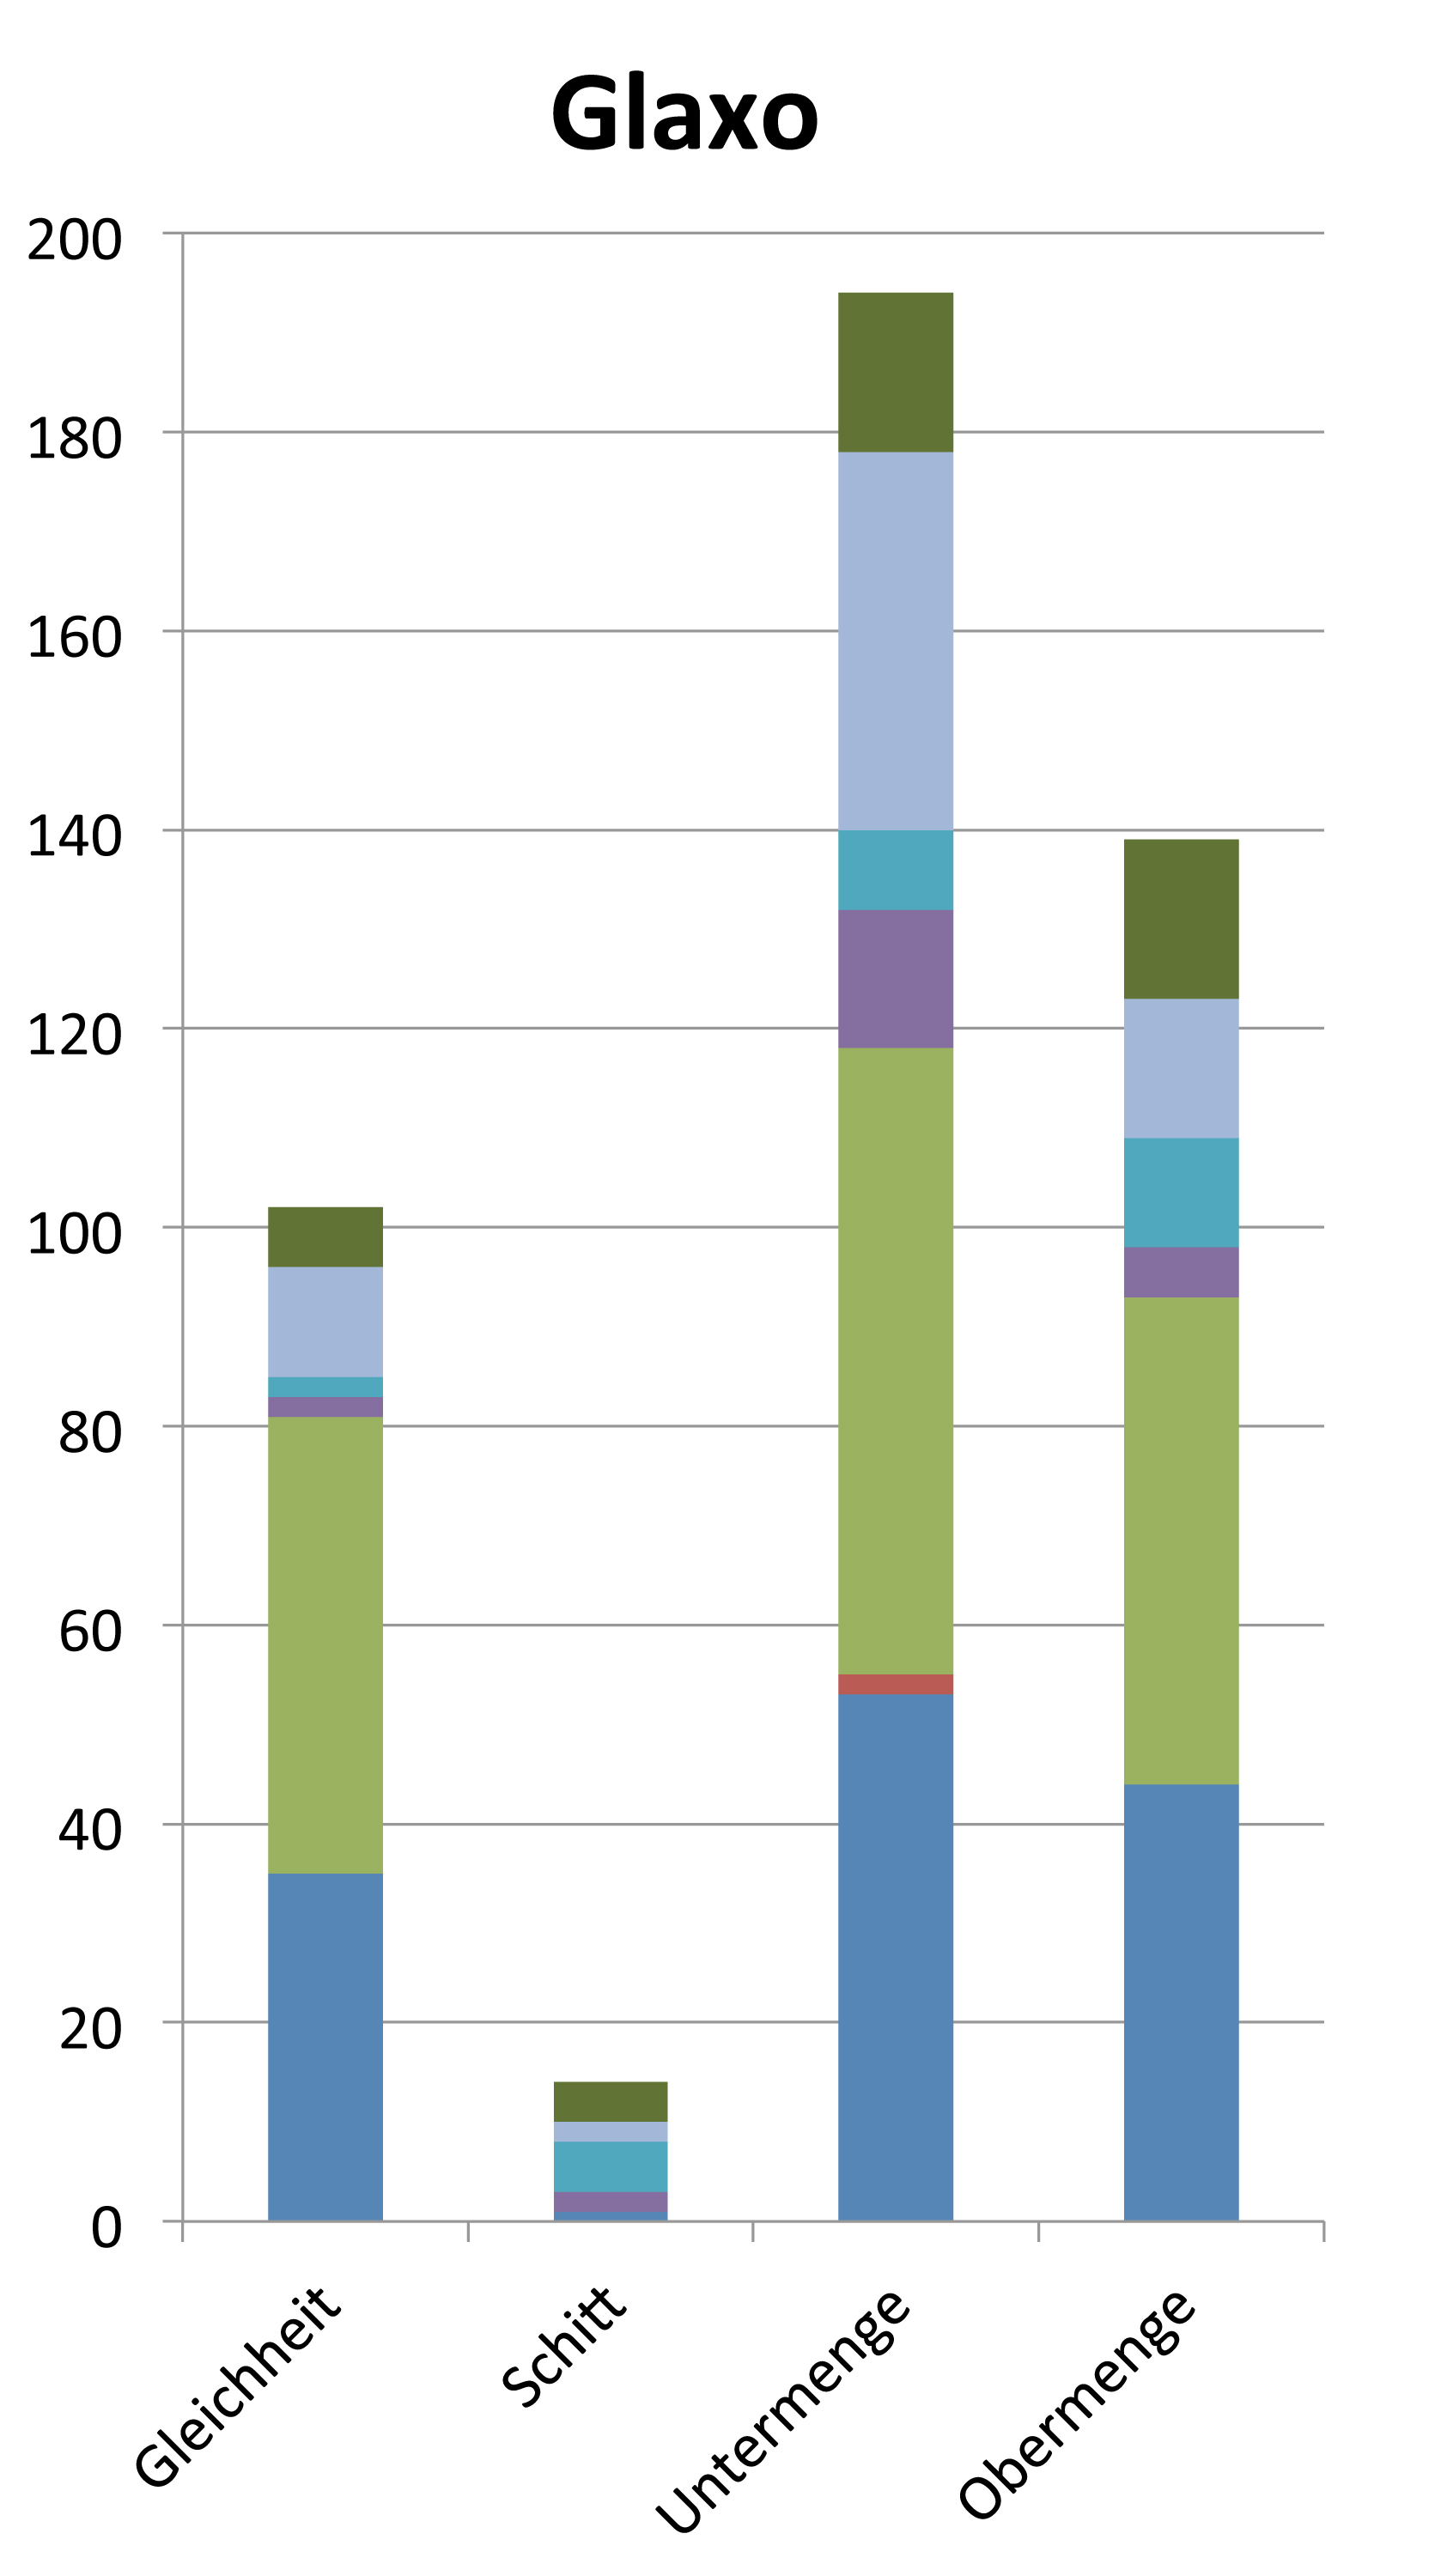
\includegraphics[width=5cm]{images/Glaxo}
	\end{minipage}
	\begin{minipage}{7cm}
		\centering
		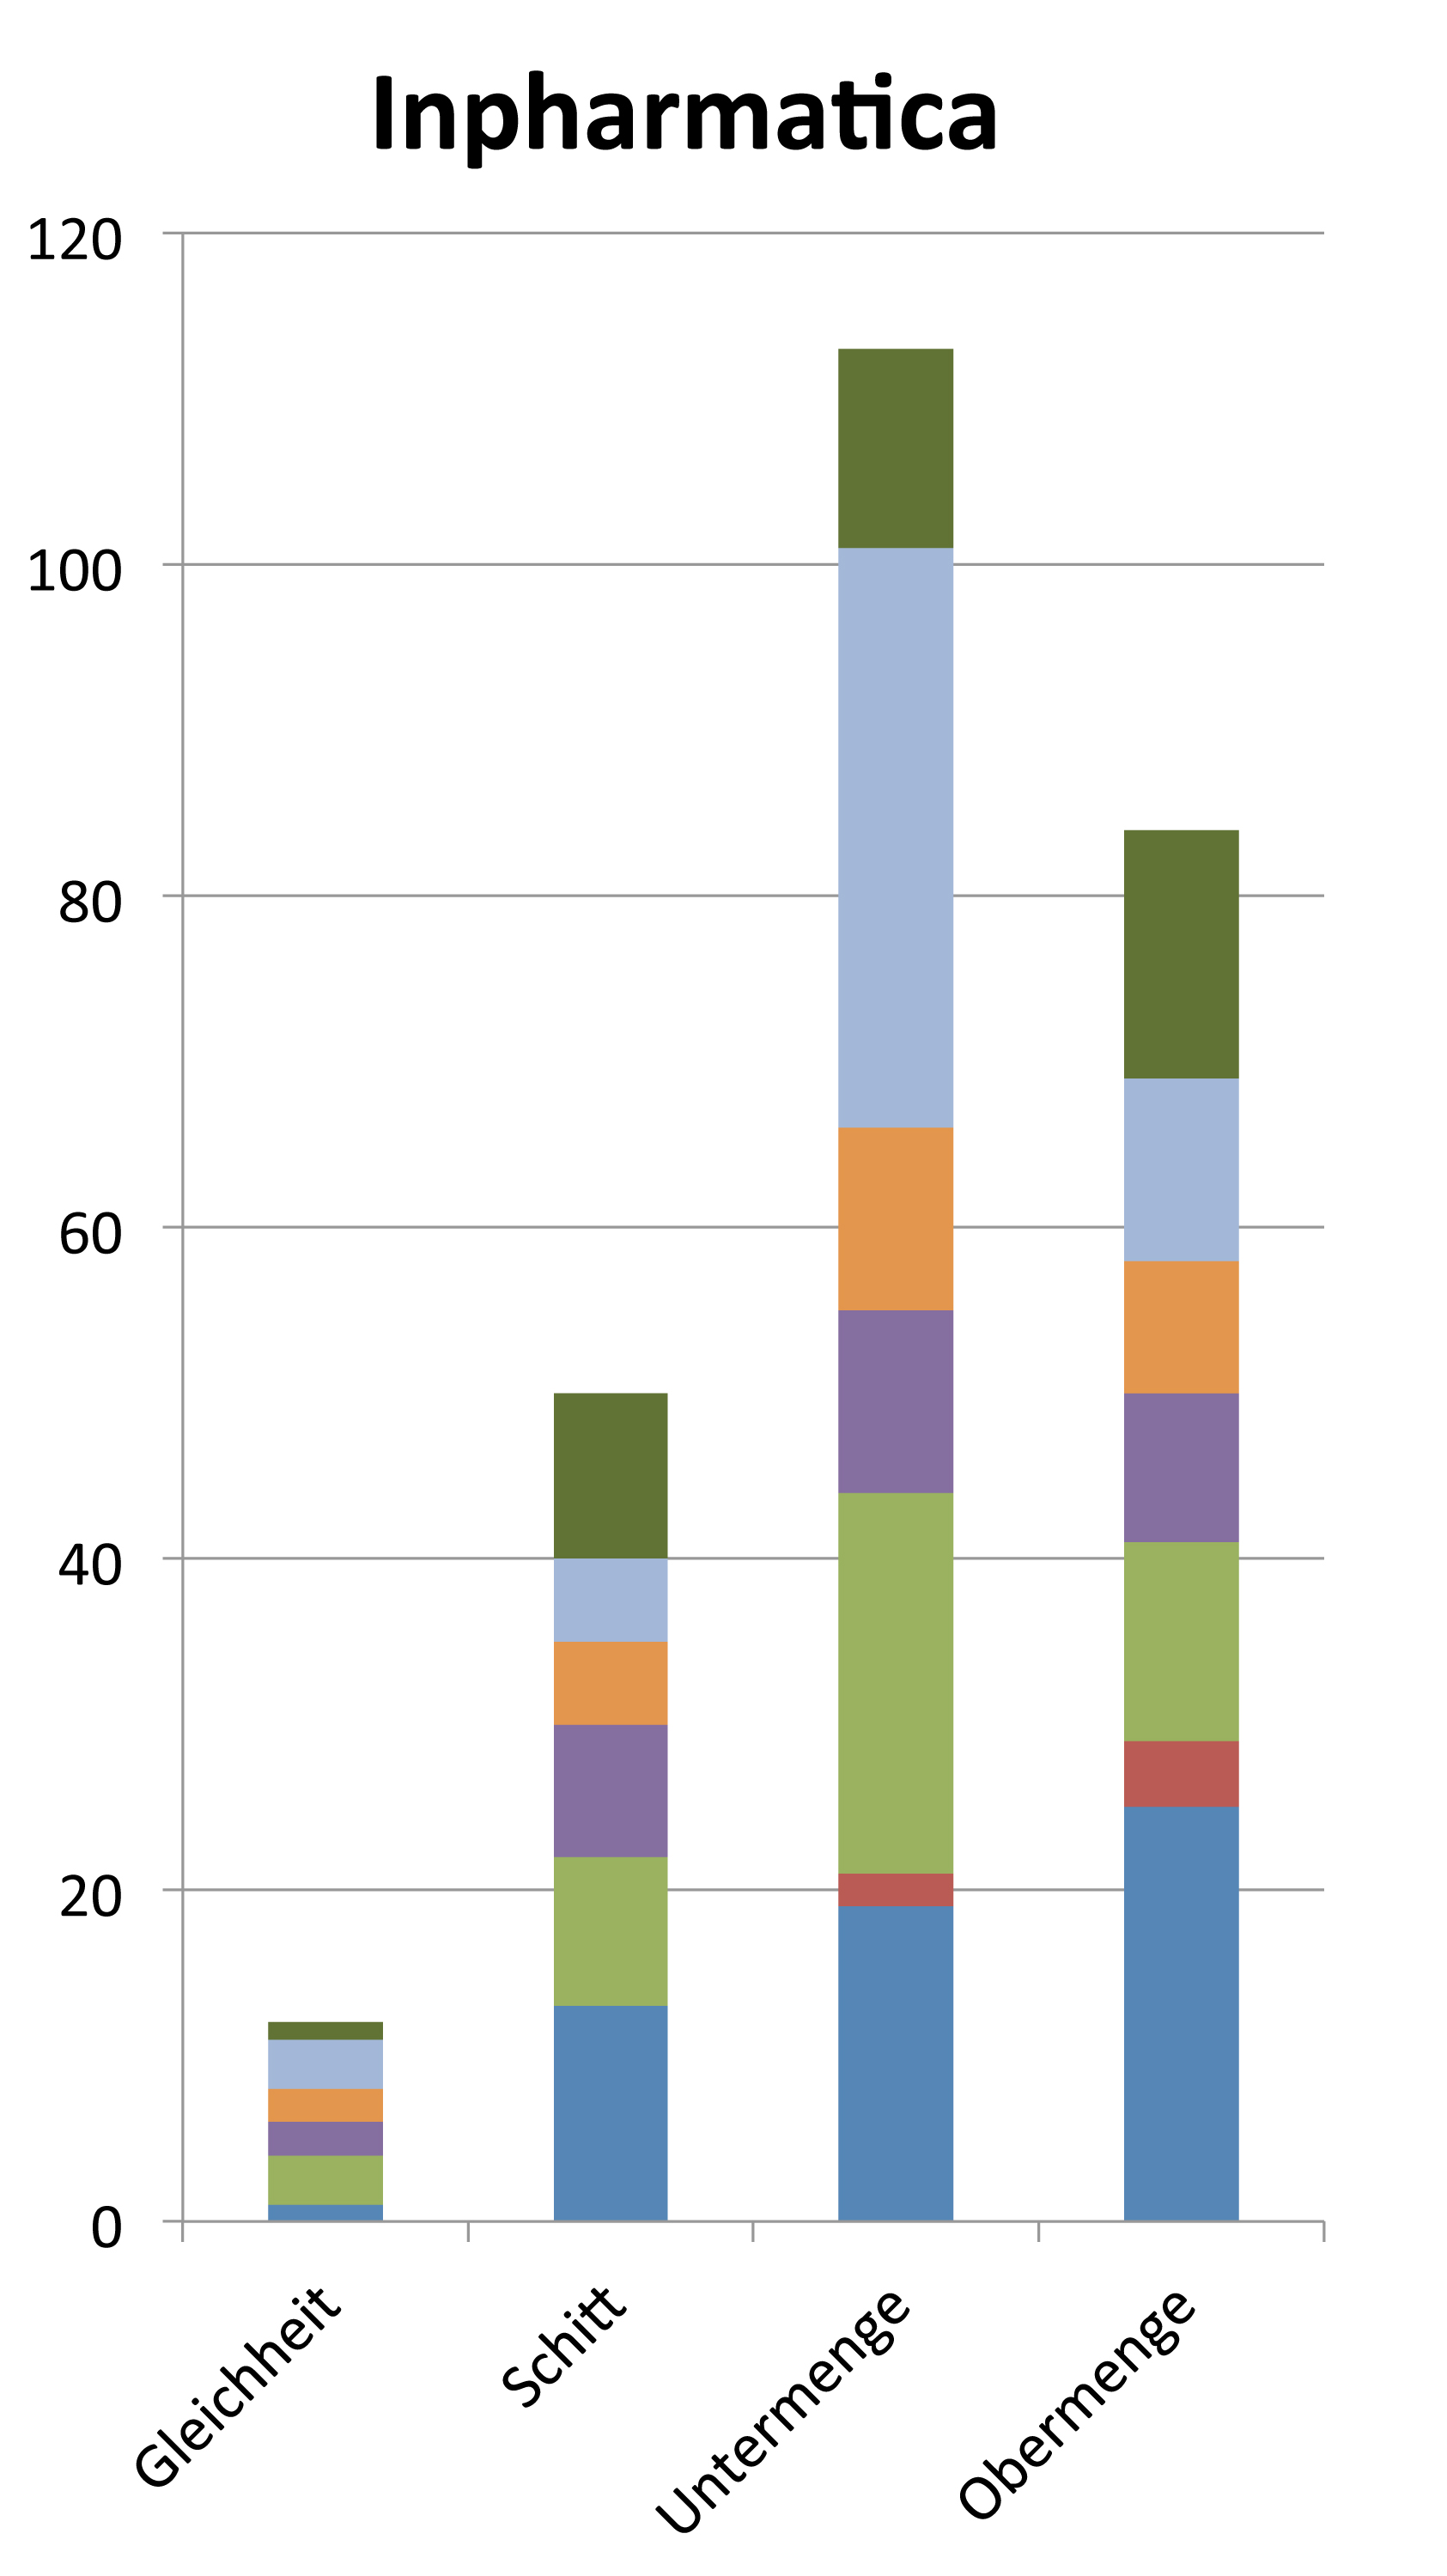
\includegraphics[width=5cm]{images/Inpharmatica}
	\end{minipage}
	\end{center}
\end{center}
\end{minipage}}
\label{abb:experiments1}
\caption{Erster Teil der Experimente: Gezeigt werden die \textit{Mapping}-Verteilungen der einzelnen SMARTS-Filter (BMS, Dundee, Glaxo und Inpharmatica). Farbig markiert sind wie viele gefundenen \textit{Mappings} aus welchen anderen Filtern stammen. Zu beachten sind die unterschiedlichen Skalierungen (vgl. Tabelle \ref{tab:experiments}).}
\end{figure}

\newpage
\subsection{Diskussion der Experimente}
Anhand der Ergebnisse die f�r die Vergleiche der Filter-Sets gewonnen wurden k�nnen R�ckschl�sse auf die Art der Sets gezogen werden. Im Folgenden wird auf die Ergebnisse von jedem Filter-Set eingegangen.

\textbf{BMS}\\
Nach Durchf�hrung der Vergleiche von dem Filter-Set von BMS mit allen anderen Filter-Sets wird deutlich, dass bei den Vergleichen vor allem eine Untermengen-Relation festgestellt wurde. Es l�sst darauf schlie�en, dass BMS im Vergleich zu den anderen (insgebsondere zu Dundee) Filter nutzt, die spezifizierter eingesetzt werden.

\textbf{Dundee}\\
Bei Dundee l�sst sich genau das Gegenteil feststellen. So sind die Filter aus diesem Set allgemeiner gehalten, als andere. 

\textbf{Glaxo}\\
Bei den Vergleichen mit dem Set von Glaxo wurden �ber 100 \textit{Mappings} gefunden, die eine Gleichheit darstellen. 

\textbf{Inpharmatica}\\
F�r Inpharmatica wurden beinahe ausgewogen Ober- und Untermengen-\textit{Mappings gefunden}.

\newpage
\begin{figure}[h!]
\fbox{\begin{minipage}{16cm}
	\begin{center}
		\begin{minipage}{5cm}
			\centering
			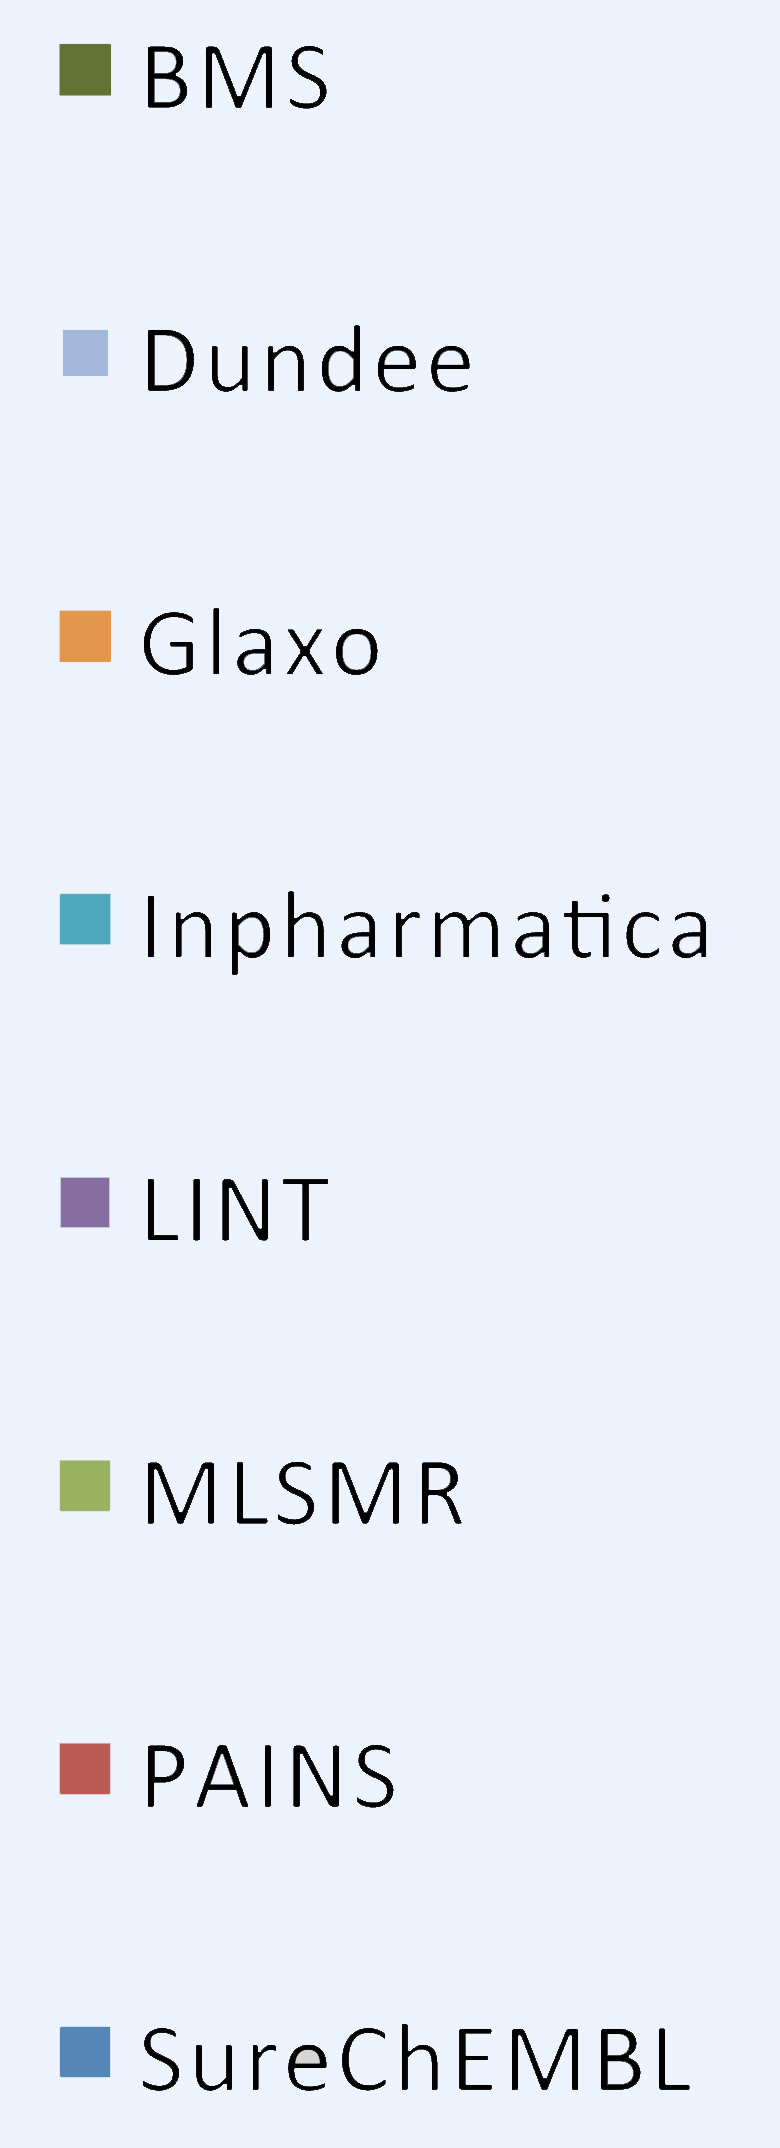
\includegraphics[width=3cm]{images/Legende3}
		\end{minipage}
		\begin{minipage}{5cm}
			\centering
			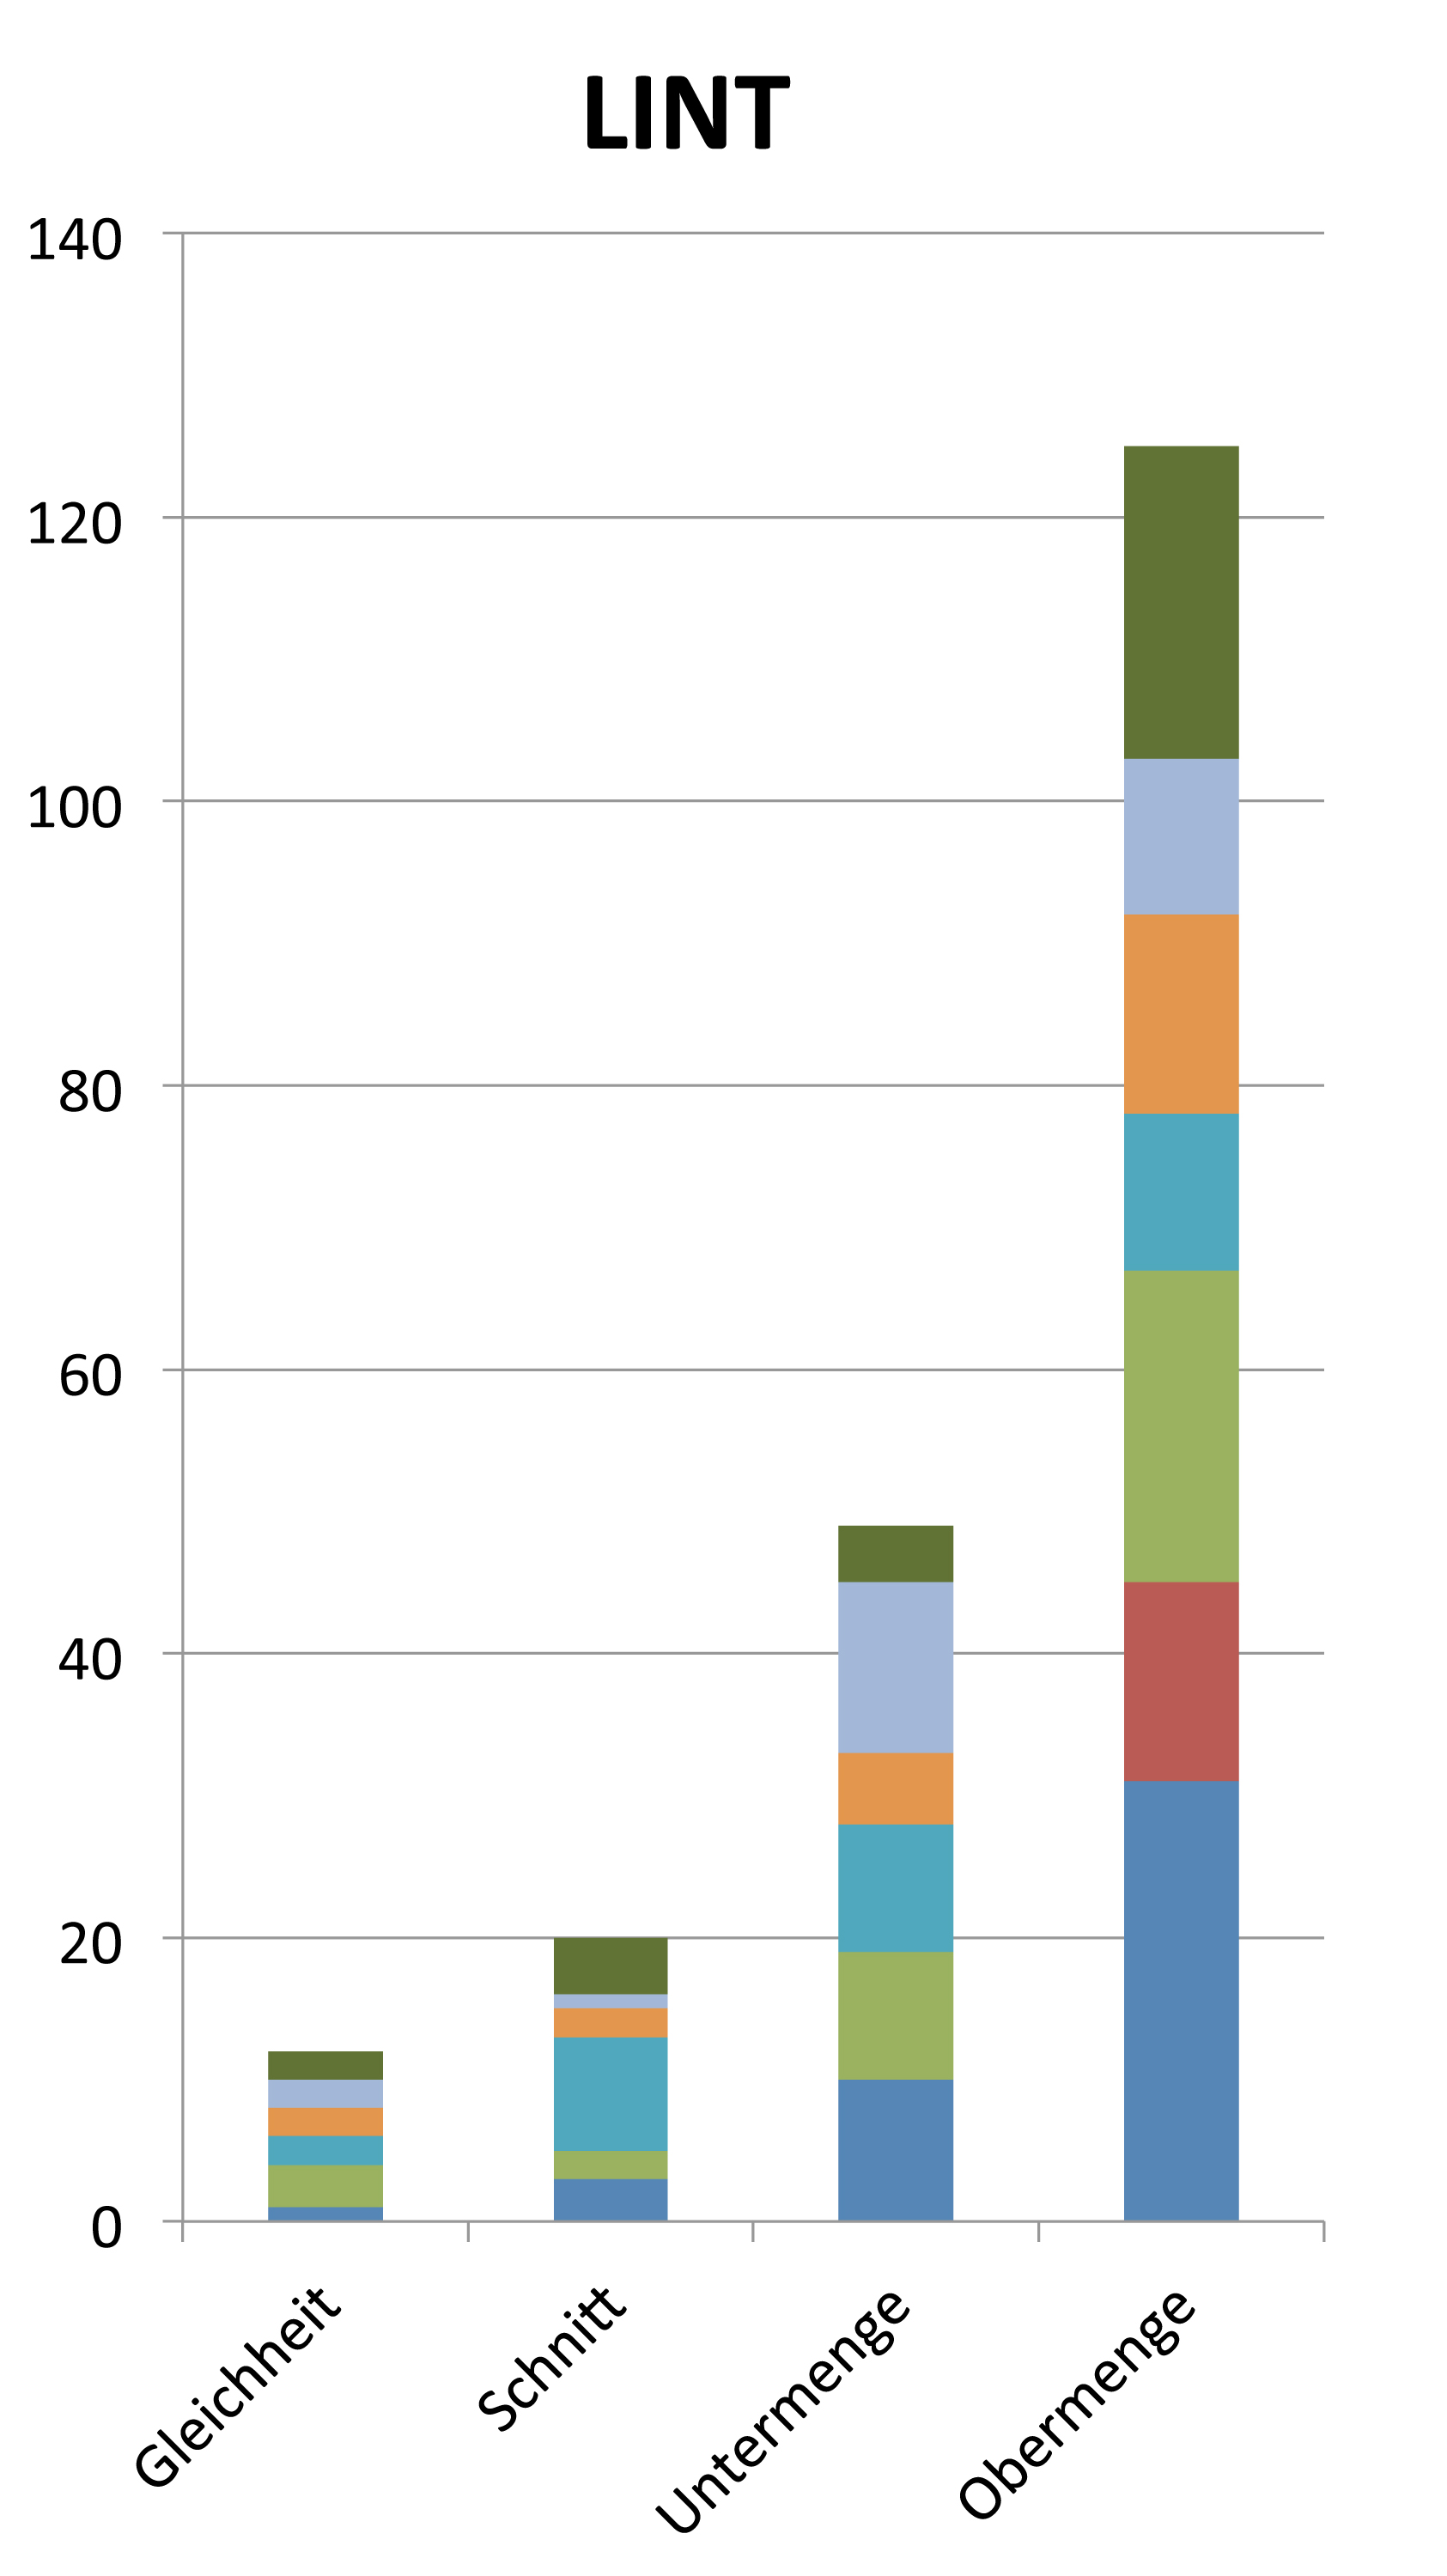
\includegraphics[width=5cm]{images/LINT}
		\end{minipage}
		\begin{minipage}{5cm}
			\centering
			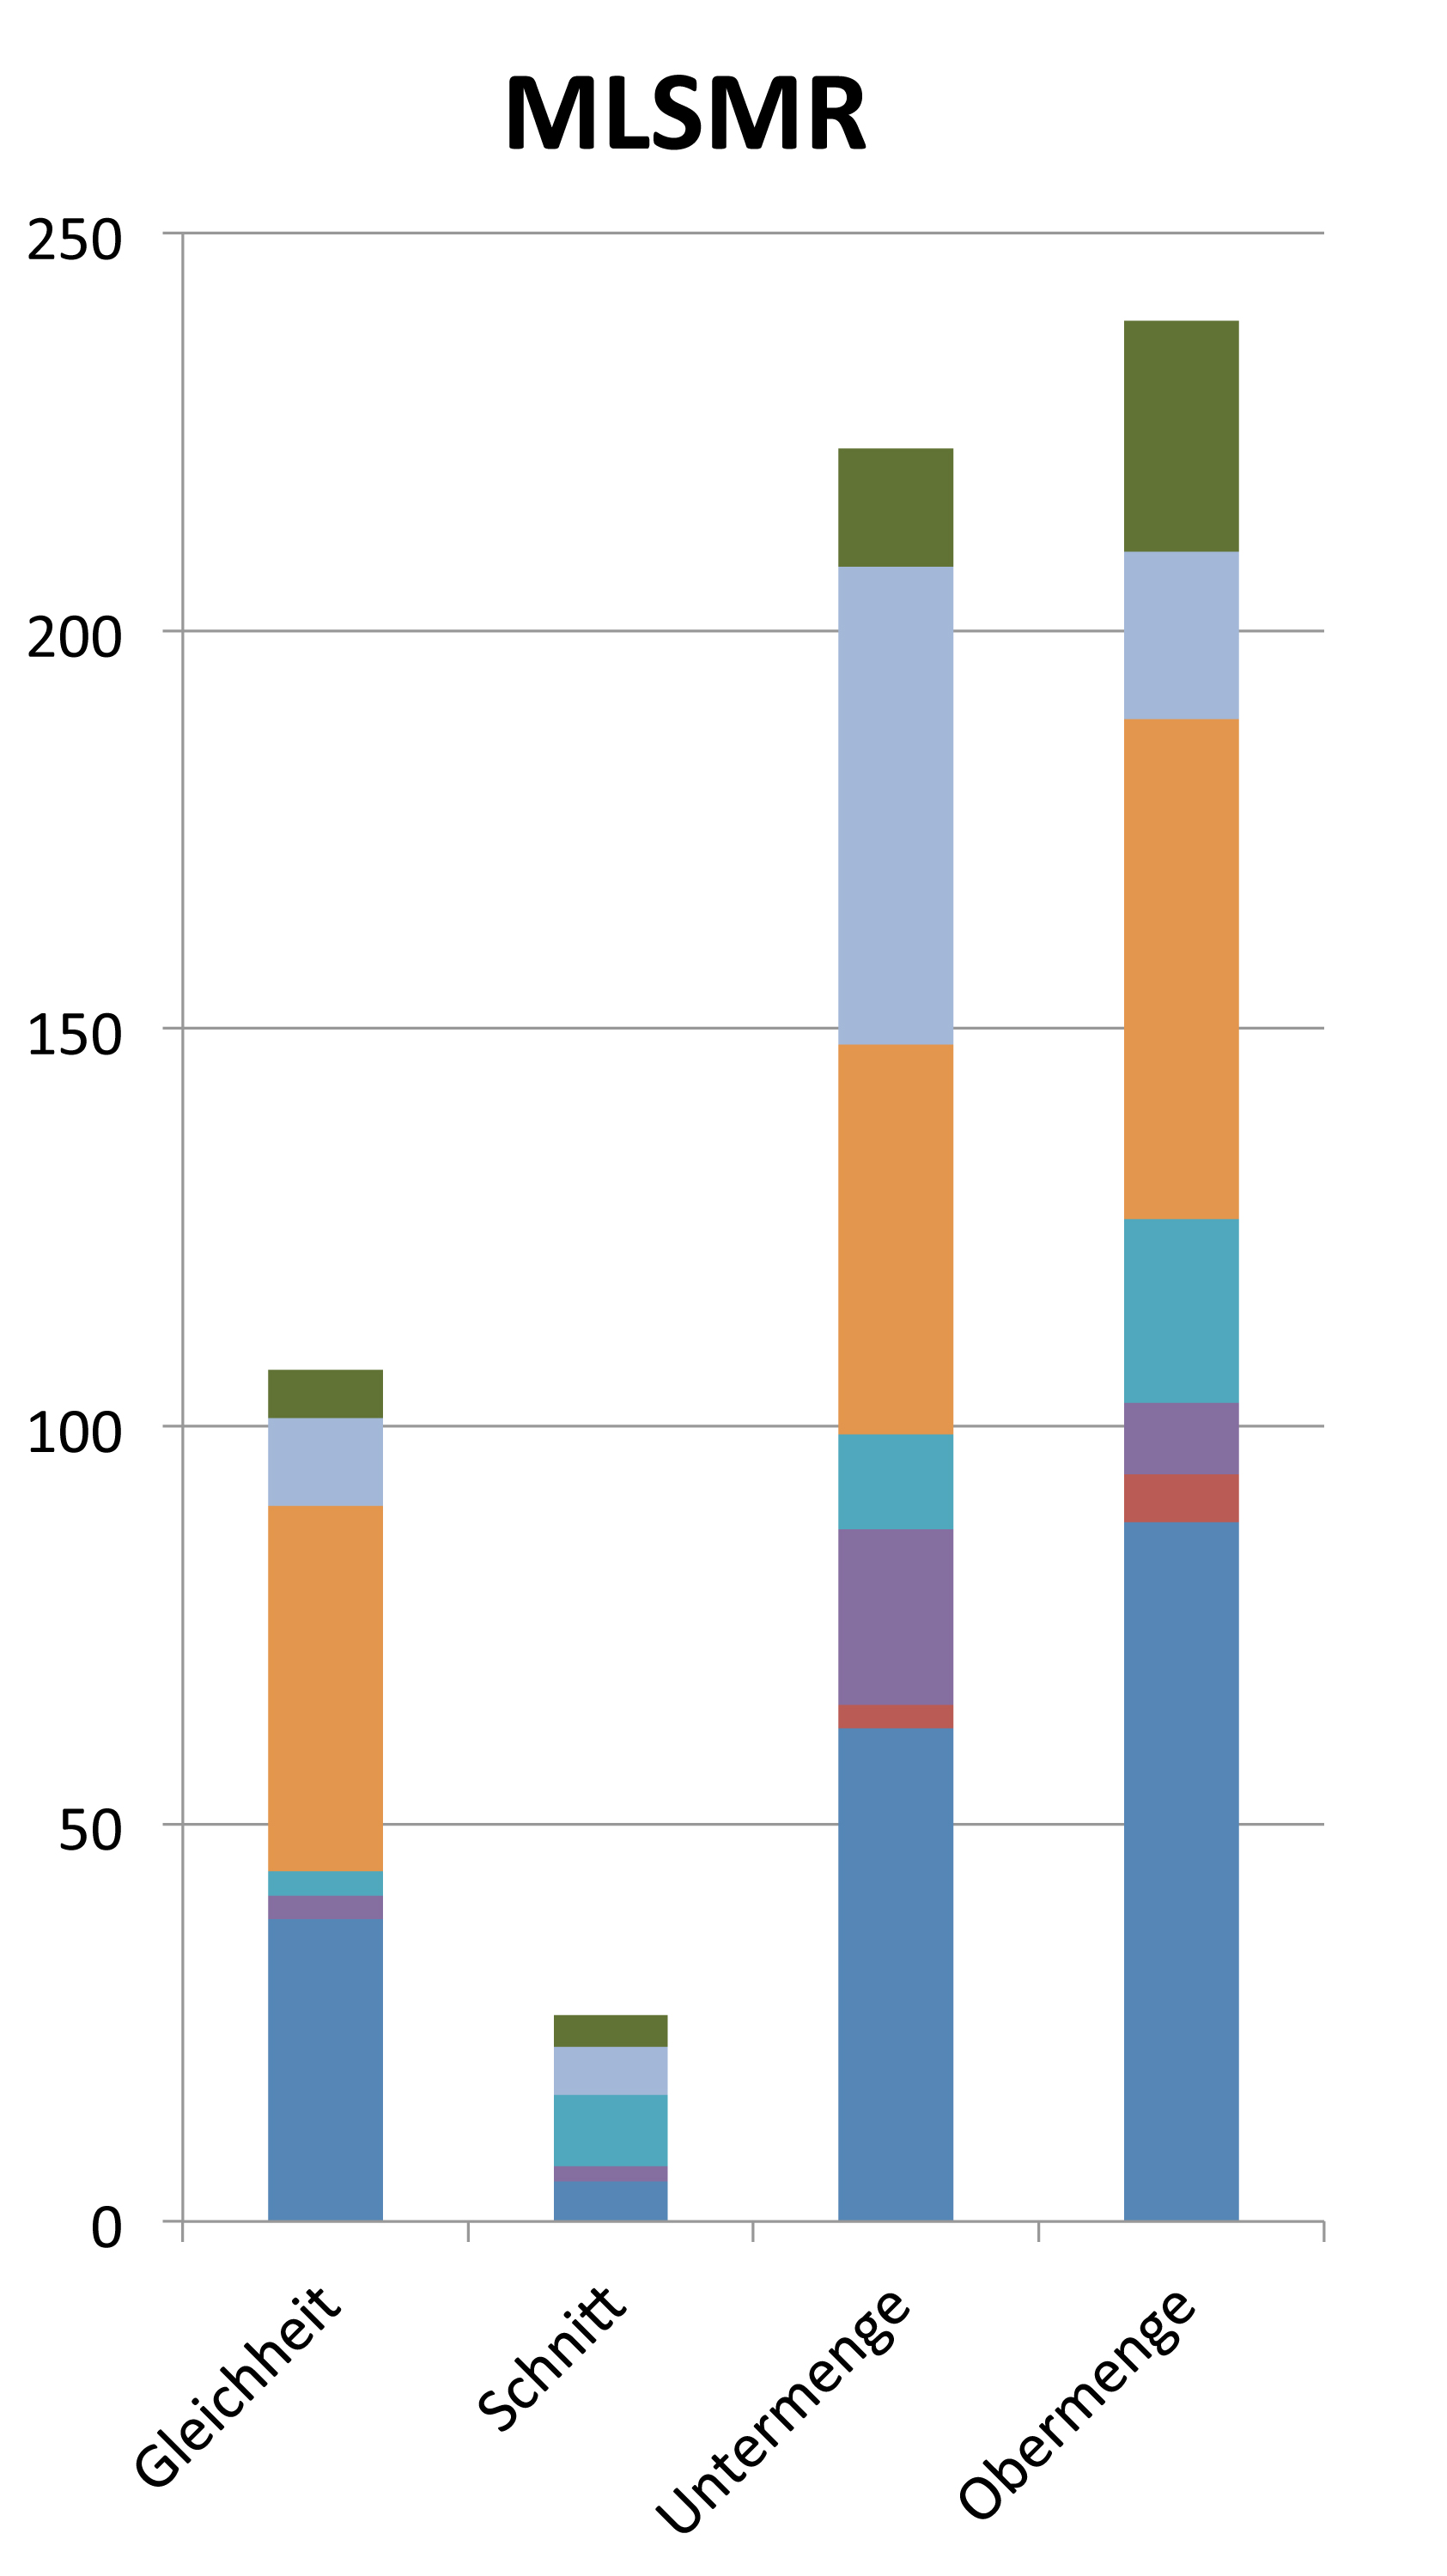
\includegraphics[width=5cm]{images/MLSMR}
		\end{minipage}
		\begin{center}
		\begin{minipage}{7cm}
			\centering
			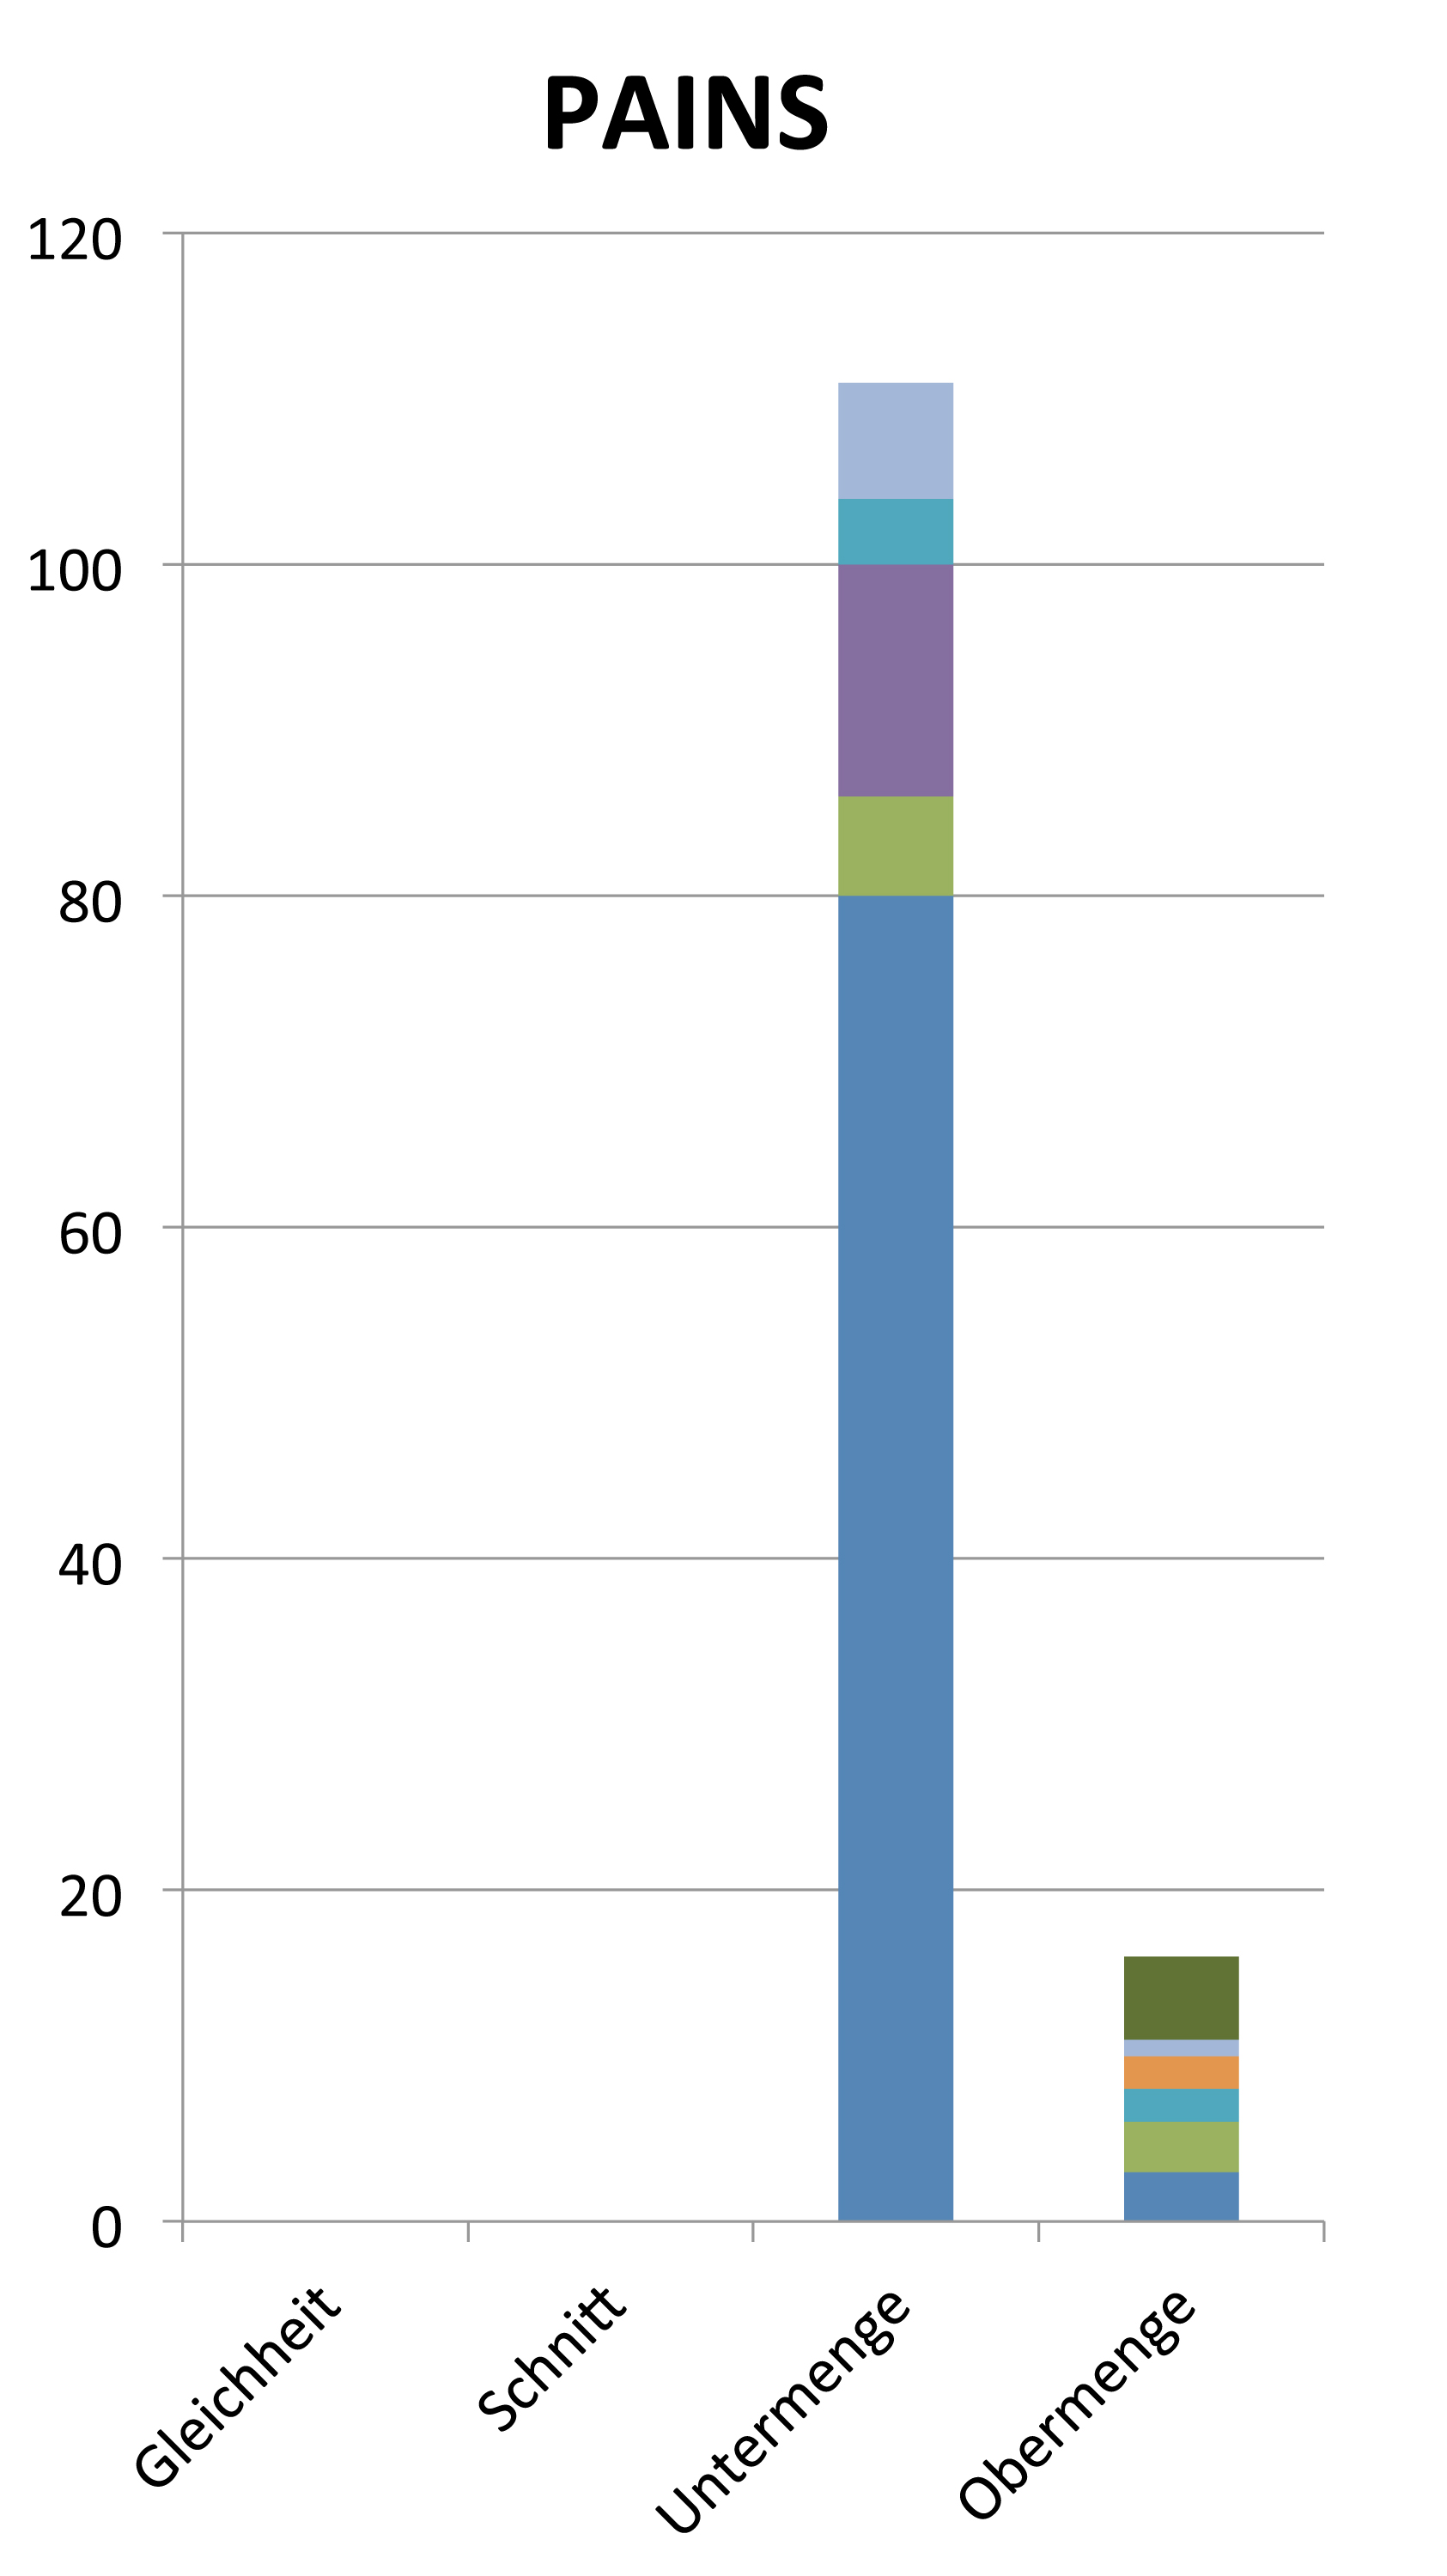
\includegraphics[width=5cm]{images/PAINS}
		\end{minipage}
		\begin{minipage}{7cm}
			\centering
			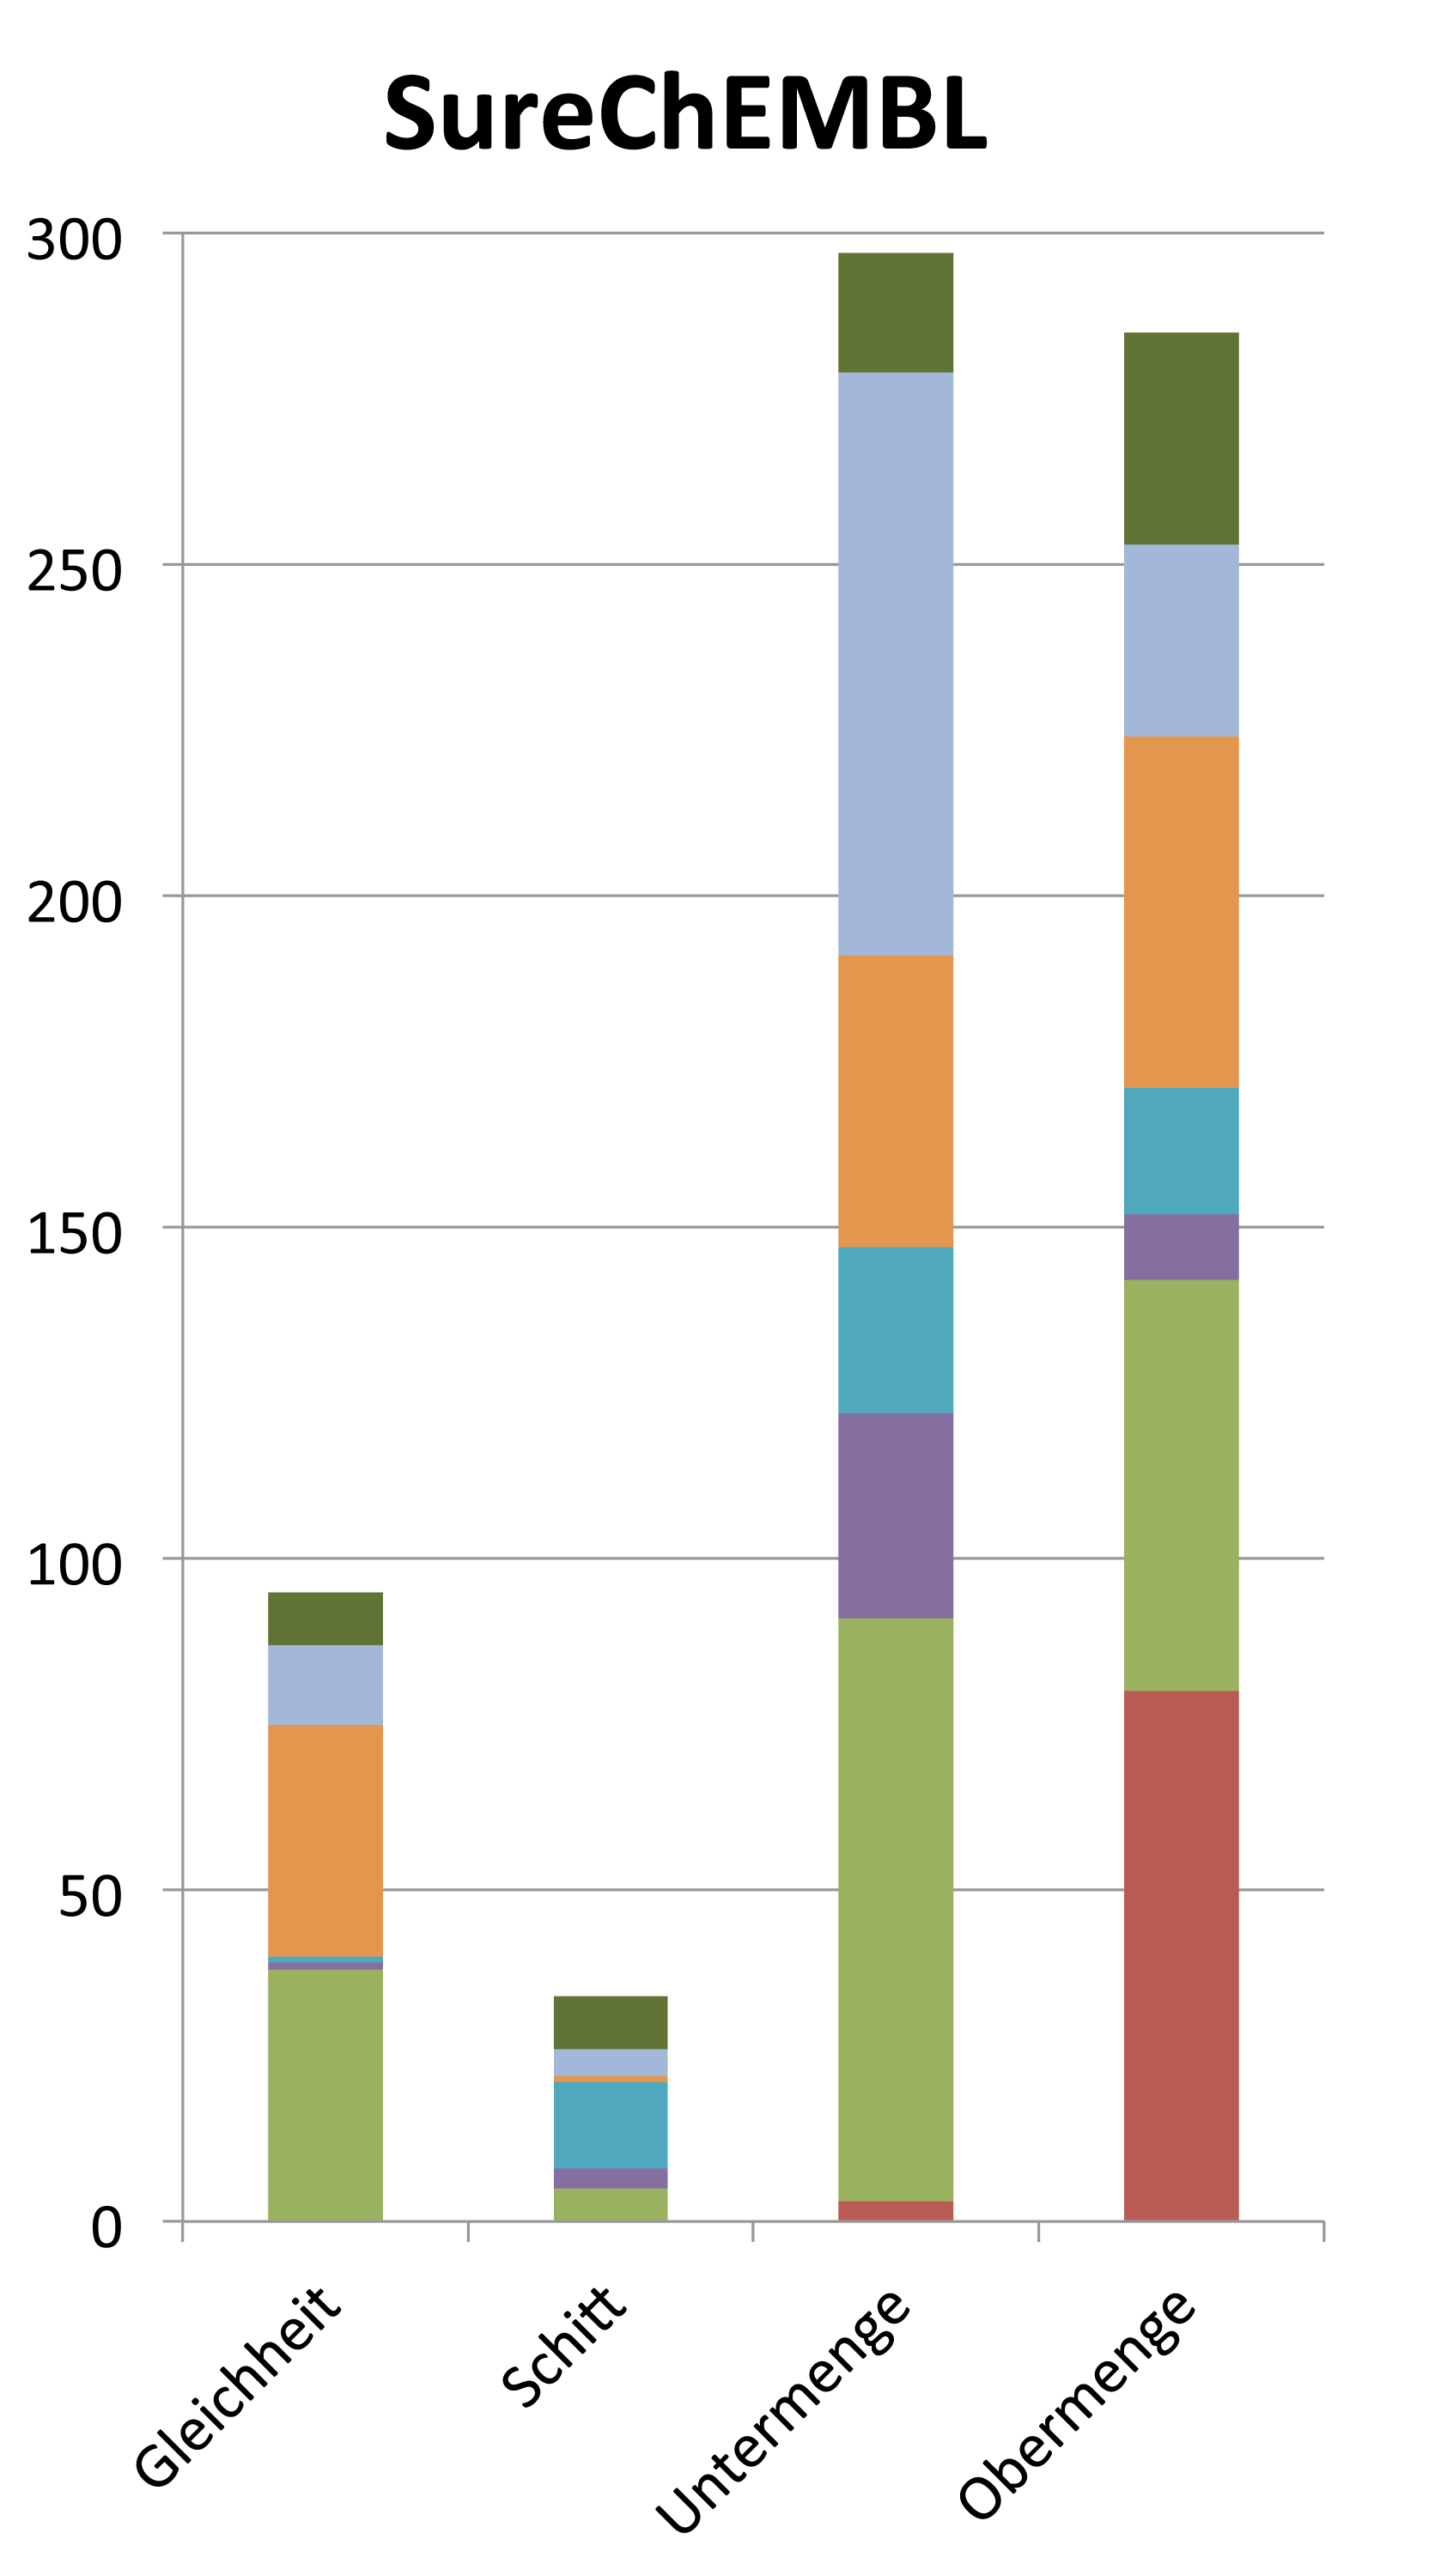
\includegraphics[width=5cm]{images/SureChEMBL}
		\end{minipage}
		\end{center}
	\end{center}
\end{minipage}}
\label{abb:experiments2}
\caption{Zweiter Teil der Experimente: Gezeigt werden die \textit{Mapping}-Verteilungen der einzelnen SMARTS-Filtern (LINT, MLSMR, PAINS, SureChEMBL). Farbig markiert sind wie viele gefundenen \textit{Mappings} aus welchen anderen Filtern stammen. Zu beachten sind die unterschiedlichen Skalierungen (vgl. Tabelle \ref{tab:experiments}).}
\end{figure}

\newpage
\textbf{LINT}\\


\textbf{MLSMR}\\


\textbf{PAINS}\\
\textbf{Hier kommt noch was}

\textbf{SureChEMBL}\\
\textbf{Hier kommt noch was}

Abschlie�end l�sst sich sagen, dass mit Hilfe des entwickelten Verfahrens sich R�ckschl�sse auf die Art der genutzten Filter-Sets ziehen lassen. So Weisen die Sets Glaxo, MLSMR und SureChEMBL eine gro�e �hnlichkeit zueinander auf. Bei anderen Sets wie LINT und Dundee wurde vor allem die Untermenge als h�ufigste Relation festgestellt, was darauf hinweist, dass diese Sets Molek�le im Vergleich grob herausfiltern. BMS und Inpharmatica hingegen, f�r die vor allem \textit{Mappings} gefunden wurden, die zu einer Obermenge geh�ren weisen darauf hin, dass Molek�leigenschaften im Vergleich zu anderen Sets spezifizierter beschrieben sind, und somit weniger Molek�le herausgefiltert werden.
%
% EOF
%